\chapter{Methods}\label{ch:methods}


\section{Probability Density Function (PDF)}
The Probability Density Function (PDF) is a concept that describes the probability of finding a particle at a certain position.
In this project, the PDF is used to track the individual trajectories of particles in phase space.
Usually this would require solving a very large number of equations.
Because solving these equations would be too costly, only the averages over the volumes in the phase space are taken using the PDF\@.
The PDF, denoted as \(f(\mathbf r_i,\mathbf v_i,t)\), represents the probability density of finding a particle at a certain position \(\mathbf{r_i}\) and velocity \(\mathbf{v_i}\) at a given time \(t\).


\section{Boltzmann Transport Equation (BTE)}
The equation formulates the evolution of motion for the PDF over time.
The Boltzmann Transport Equation (BTE) consists of two parts.
The first part is \textit{streaming} and resembles only the moving of particles.
The second part is called \textit{collision} and deals with the interaction between particles while moving.

\subsection{Streaming}\label{subsec:streaming}
The probability density of the PDF is able to move, which is described by the Boltzmann Transport Equation (BTE).
BTE transports the probability density distributions at a specific velocity in real space.
While transporting, the influence of the velocity and acceleration are considered.
The combined effect of velocity and acceleration leads to the streaming of density.
\newline

The whole Boltzmann Transport Equation is denoted as
\begin{equation}
    \frac{\partial f\left(\mathbf{r},\mathbf{v},t\right)}{\partial t}+\mathbf{v}\nabla_{\mathbf{r}} f\left(\mathbf{r},\mathbf{v},t\right)
    +\mathbf{a}\nabla_{\mathbf{v}} f\left(\mathbf{r},\mathbf{v},t\right)=C(f)
    \cdot
    \label{eq:bte}
\end{equation}

The l.h.s.\ of the equation denotes the streaming part that was just explained and the r.h.s.\ the collision, explained in the following part.

\subsection{Collision}\label{subsec:collision}
Only applying streaming resembles a probability of collision of 0\%, which is not realistic.
To account for collisions, an additional term is introduced into the equation to represent the collision process that occurs at each time step.
In reality, collisions between particles result in an almost instantaneous exchange of energy and momentum.
However, these collisions occur in extremely short time intervals on the order of femtoseconds (\(10^{-15}\) seconds), making it impractical to measure them directly in the model.
Therefore, the collision process is approximated as an instantaneous process.
Because of this instantaneous, it cannot be represented as a differential equation, which normally describes continuous changes.
Instead, a probabilistic approach is taken to describe the effects of collisions.
\newline

In the previous ~\cref{subsec:streaming}, the Boltzmann Transport Equation (BTE) was introduced (\cref{eq:bte}), where the right term represents the collision process.
To simplify this collision term, a relaxation time approximation is commonly used.
This approximation assumes that the probability density function (PDF) \(f\left(\mathbf{r},\mathbf{v},t\right)\) relaxes towards a local equilibrium distribution, denoted as \(f^{eq}\left(\mathbf{r},\mathbf{v},t\right)\).
By interpreting the streaming term as the total time derivative of the PDF, the BTE can be reformulated as follows:

\begin{equation}
    \frac{d}{dt} f\left(\mathbf{r},\mathbf{v},t\right) = -\frac{ f\left(\mathbf{r},\mathbf{v},t\right)- f^{eq}\left(\mathbf{r},\mathbf{v},t\right)}{\tau}
    \cdot
    \label{eq:bgk}
\end{equation}

The included equilibirum function can is denoted as
\begin{equation}
    f_i^{eq}(\rho(\mathbf{r}),\mathbf{u}(\mathbf{r}))
    =w_i\rho(\mathbf{r})
    \left[
        1+3\mathbf{c}_i\cdot\mathbf{u}(\mathbf{r})
        +\frac{9}{2}\left(\mathbf{c}_i\cdot\mathbf{u}(\mathbf{r})\right)^2
        -\frac{3}{2}|\mathbf{u}(\mathbf{r})|^2
        \right]
    \cdot
    \label{eq:feq}
\end{equation}

The equilibrium function introduces some additional quantities, namely the density \(\rho(\mathbf{r})\), velocity \(\mathbf{u}(\mathbf{r})\) and \(w_i\).
\(w_i\) is defined for a D2Q9 lattice as seen in~\cref{eq:w}.
The other two quantities can be calculated using the following formulas.
\begin{equation}
    w_i = \left(\dfrac{4}{9},
    \dfrac{1}{9}, \dfrac{1}{9}, \dfrac{1}{9}, \dfrac{1}{9},
    \dfrac{1}{36}, \dfrac{1}{36}, \dfrac{1}{36}, \dfrac{1}{36}\right)
    \label{eq:w}
\end{equation}
\begin{equation}
    \rho(\mathbf{r})=\sum_i f_i
    \label{eq:rho}
\end{equation}
\begin{equation}
    \mathbf{u}(\mathbf{r})=
    \frac{1}{\rho(\mathbf{r})}\sum_i \mathbf{c}_i f_i(\mathbf{r})
    \label{eq:u}
\end{equation}


\section{Lattice Bolzmann Scheme}\label{sec:lattice-bolzmann-scheme}

In order to discretize the Boltzmann Transport Equation (BTE), it is necessary to incorporate both velocity and position space into the discrete scheme representation.
An effective approach involves utilizing a 2D grid, as illustrated in \cref{fig:bte-scheme}.
The grid represents the position space as coordinates of the x and y coordinates.
\newline

Each position holds a probability density value, resembled by the value at that point.
The velocities are included when introducing a third dimension, that separates the different streaming directions.
To get the probability density function back, only the sum of all different directions in one point is needed.
The probability density function can be reconstructed by simply summing the values for all different directions at a given point.
\newline

The streaming, as explained in \cref{subsec:streaming}, is applied by moving the values of the points in one of 9 directions in their respective dimension.
The collision process can be implemented by employing the functions described in \cref{subsec:collision}.
During collisions, densities may be transferred between different dimensions within the scheme.

\begin{figure}[H]
    \begin{center}
        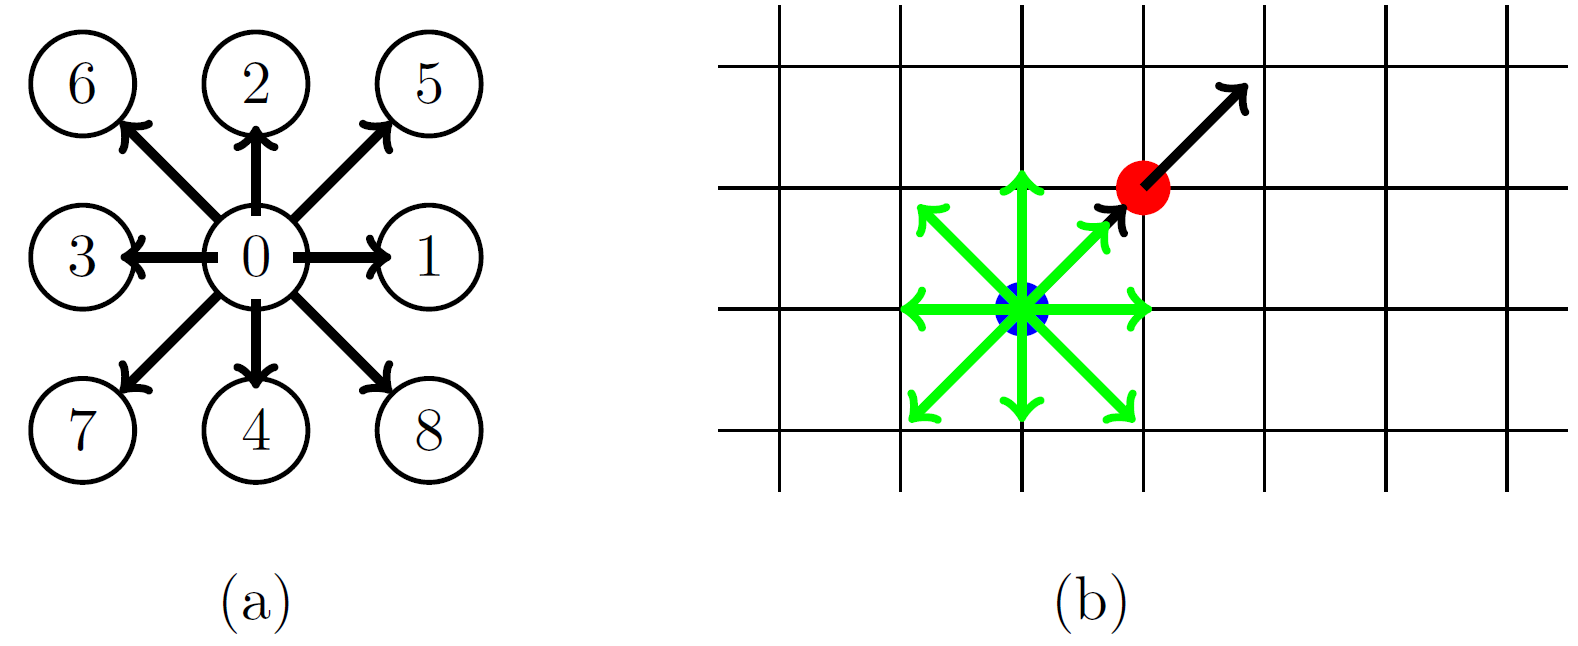
\includegraphics[width=10cm]{logos/Gitter_LBM.png}
        \caption[Visualization of the underlying grid including labled directions.]{
            Visualization of the underlying grid including labled directions. \\
            (a) directions with given labels \\
            (b) streaming example of one particle
        }
        \label{fig:bte-scheme}
    \end{center}
\end{figure}
